% Created 2017-11-02 Thu 21:04
% Intended LaTeX compiler: pdflatex
\documentclass[11pt]{article}
\usepackage[utf8]{inputenc}
\usepackage[T1]{fontenc}
\usepackage{graphicx}
\usepackage{grffile}
\usepackage{longtable}
\usepackage{wrapfig}
\usepackage{rotating}
\usepackage[normalem]{ulem}
\usepackage{amsmath}
\usepackage{textcomp}
\usepackage{amssymb}
\usepackage{capt-of}
\usepackage{hyperref}
\usepackage{amsmath}
\author{Jake Brawer}
\date{\today}
\title{Assignment 5}
\hypersetup{
 pdfauthor={Jake Brawer},
 pdftitle={Assignment 5},
 pdfkeywords={},
 pdfsubject={},
 pdfcreator={Emacs 25.2.1 (Org mode 9.1.2)}, 
 pdflang={English}}
\begin{document}

\maketitle

\section*{Problem 1}
\label{sec:org8d568f5}
Let \(X\) be Katie's choice of path and \(Y\) be Pele's. Then\\
\begin{equation}
  \begin{aligned}
    E(T) &= \sum_{X}^{}\sum_{Y}^{}E(T | X = x, Y = y)P\{X = x\}P\{Y = y\} \\
    &=\frac{1}{9} \biggl( E(T | AB,BA) + E(T | AB,BC) + E(T | AB,BD)  \\
      & \qquad + E(T | AC,BA) + E(T | AC,BC) + E(T | AC,BD)   \\
      & \qquad + E(T | AD,BA) + E(T | AD,BC) + E(T | AD,BD) \biggr) \\
    &= \frac{1}{9} \biggl( \frac{1}{2} +  (1 + E(T)) +  (1 + E(T))\\
      & \qquad + (1 + E(T)) + 1 +  (1 + E(T))\\
      & \qquad + (1 + E(T)) + (1 + E(T)) + 1 \biggr)\\
      &= \frac{1}{9} \left( 2.5 +  6(1 + E(T)) \right)\\
      &= \frac{8.5}{9} + \frac{2}{3}E(T)\\
      &= \frac{8.5}{3}
  \end{aligned}
\end{equationn}

\section*{Problem 2}
\label{sec:org355f764}
\subsection*{a)}
\label{sec:orgf3ab86c}
Let \(X_{T}\) denote the number of umbrellas at the current location before 
trip \(T\). So \(S = \{0,1,2,3,4\}\). Let \(P\) be a transition matrix associated with
\(X_{T}\). So:

P= 
\begin{bmatrix}
  0 & 0 & 0 & 1\\
  0 & 0 & .8 & .2\\
  0 & .8 & .2 & 0\\
  .8 & .2 & 0 & 0
\end{bmatrix}

\subsection*{b)}
\label{sec:orge2af3b4}

\begin{align}
  \pi P = \pi \\
  \rightarrow & \pi_{0} = .8\pi_{3}\\
               & \pi_{1} = .8\pi_{2} + .2\pi_{3}\\
              & \pi_{2} = .8\pi_{1} + \pi_{2}\\
              & \pi_{3} = .8\pi_{0} + \pi_{1}\\
\end{align}

From here we get:\\

\begin{align*}
  \pi_{3} = \pi_{1} \tag{by (6)} \\
  \pi_{2} = \pi_{1} \tag{from (5)}\\
  \text{So: } \pi_{3} = \pi_{2}.
\end{align*}

So \pi =\[.8\pi_{3}, \pi_{3},  \pi_{3},  \pi_{3} \]\\
\begin{align*}
  \text{We know that } \sum_{i}^{} \pi_{i} &= 1 = 3.8\pi_{3}\\
\end{align*}

So $\pi_{3} = \frac{5}{19}$ and our stationary distribution is: \\
\begin{equation*}
  \pi = \left[\frac{4}{19}, \frac{5}{19}, \frac{5}{19},\frac{5}{19} \right]
\end{equation*}

\subsection*{c)}
\label{sec:org061dda4}
\begin{verbatim}
matpow = function (M,n) {
# Finds matrix power M^n.
# Use this for n = integer greater than 1.
  ans = M
  for(i in 1:( n-1 )) {
    ans = ans %*% M
  }
  return (ans)
}

P = matrix(c(0,0,0,1,
             0,0,.8,.2,
             0,.8,.2,0,
             .8,.2,0,0), byrow=TRUE, ncol=4)

matpow(P,1000)

\end{verbatim}

\begin{center}
\begin{tabular}{rrrr}
0.21052631578948 & 0.26315789473685 & 0.263157894736849 & 0.263157894736849\\
0.21052631578948 & 0.26315789473685 & 0.26315789473685 & 0.26315789473685\\
0.210526315789479 & 0.263157894736849 & 0.263157894736849 & 0.263157894736849\\
0.21052631578948 & 0.263157894736849 & 0.26315789473685 & 0.26315789473685\\
\end{tabular}
\end{center}

My calculated stationary dist:
\begin{verbatim}
matrix(c(4/19,5/19,5/19,5/19), byrow=TRUE,ncol=4)
\end{verbatim}

\begin{center}
\begin{tabular}{rrrr}
0.210526315789474 & 0.263157894736842 & 0.263157894736842 & 0.263157894736842\\
\end{tabular}
\end{center}

\subsection*{d)}
\label{sec:org82d8e17}
Fred only gets wet when he's in state zero (i.e. he's at a location with no umbrellas)
and it starts to rain (with \(0.2\) probability) so:\\
\begin{equation*}
  \pi(0)P_{rain} = .21 * 0.2 = .0421
\end{equation*}

\section*{Problem 3}
\label{sec:org2d4e683}
\subsection*{a)}
\label{sec:orgc42e885}
We can show that this is not a Markov chain by proving that the Markov property 
does not hold. The Markov property states that 
\begin{equation*}
  P(X_n=x_n\mid X_{n-1}=x_{n-1}, \dots, X_0=x_0)=P(X_n=x_n\mid X_{n-1}=x_{n-1}). 
\end{equation*}
From the problem its clear to see that $S = \{-1, 0, 1\}$\\
Let $X_{0} = 1$ $X_{0}^{*} = -1$  be the starting states of two chains and
$X_{1} = 0$ be an intermediary state shared by both.\\
We want to see if $$P\{X_{2} = x_{2} | X_{1} = x_{1}, X_{0} = x_{0}\} =
P\{X_{2} = x_{2} | X_{1} = x_{1}, X_{0}^{*} = x_{0}^{*}\}$$.\\
The LHS sequence of $Y$s must be:
\begin{equation*}
  Y_{-1} = 1, Y_{0} = 1, Y_{1} = -1
\end{equation*}
And the RHS must be:
\begin{equation*}
  Y_{-1} = -1, Y_{0} = -1, Y_{1} = 1
\end{equation*}
Given that $X_{2} = \frac{1}{2}(Y_{1} + Y_{2})$\\
\begin{equation*}
  P\{X_{2} = 1 | X_{1} = 0, X_{0} = 1\}\ \neq P\{X_{2} = 1 | X_{1} = 0, X_{0}^{*} = -1\}\
\end{equation*}

Because $X_{2} \neq 1$ if $X_{0} = 1$ but can if $X_{0} = -1$. Thus the Markov property does not hold.

\subsection*{b)}
\label{sec:org97b7989}
Let $X_{0} = 1$ $X_{0}^{*} = -1$  be the starting states of two chains and
$X_{1}...X_{r -1} = 0$ be subsequent states shared by both chains. For the
chain starting at $X_{0} = 1$ all $Y_{odd} = -1, Y_{even} = 1$. For the chain
starting at $X_{0}^{*} = 1$ all $Y_{odd} = 1, Y_{even} = -1$. This means that
$Y_{r}^{*} \neq Y_{r} \forall r$  and thus that
$$P\{X_{r} =  x_{r}| X_{r - 1} = x_{r-1}, \dots X_{0} = x_{0}\} \neq  P\{X_{r} =
x_{r}| X_{r-1} = x_{r-1}, \dots X_{0}^{*} = x_{0}^{*}\}$$

\section*{Problem 4}
\label{sec:orgc5c1427}
\subsection*{a)}
\label{sec:orgdc51192}
P =
\begin{bmatrix}
  1-a & a\\
  b & 1-b\\
\end{bmatrix}

\begin{align}
  \pi P = \pi \\
  \rightarrow & \pi_{1} = (1 - a)\pi_{1} + \pi_{2}b\\
              & \pi_{2} = \pi_{1}a + \pi_{2}(1-b)\\
\end{align}

From $(1)$ we get:\\
\begin{align*}
  \pi_{1} &= \pi_{1} - \pi_{1}a + \pi_{2}b\\
          &= \frac{\pi_{2} b}{a}
\end{align*}

Plugging this into $(2)$ we get:\\
\begin{align*}
  \pi_{2} &= \pi_{2}b + \pi_{2} - \pi_{2}b\\
          &= \pi_{2}
\end{align*}

So: $\sum_{i}\pi = 1 = \frac{\pi_{2}b}{a} + \pi_{2}$\\
Solving for $\pi_{2}$ we get $\pi_{2} = \frac{a}{a+b}$\\
And thus: $\pi = \left[ \frac{b}{a+b}\, \frac{a}{a+b}\right]$

\subsection*{b)}
\label{sec:org6bfd45e}
\begin{verbatim}

a <- 1/2
b <- 1/3

b/(a+b)
P = matrix(c(1-a, a,
             b, 1-b), byrow=TRUE, ncol=2)

p100  <- matpow(P,100)
sprintf("Prob that 100th question is true: %s", p100[1])
\end{verbatim}

\begin{verbatim}
Prob that 100th question is true: 0.4
\end{verbatim}

\subsection*{c)}
\label{sec:org5f96859}

\begin{verbatim}
simExam <- function(sz, P){
  # Here 1 == TRUE, 2 == FALSE
  start <- sample(1:2,size=1, prob = c(1/2,1/2))
  numTrue <- if(start == 1) 1 else 0
  prev <- start
  for(i in 2:sz)
  {
    prev <- sample(1:2, size = 1, prob = P[prev, ])
    numTrue <- if(prev == 1) numTrue + 1 else numTrue
  }
  return(numTrue / sz)
}

reps <- 1000
size <- 100
tsts <- rep(0, reps)
for(i in 1:reps){
  tsts[i] <- simExam(size, P)
}
sd(tsts)
mean(tsts)
sprintf("After %s exams: \n\t mean frac. of TRUEs: %s \n\t SD of TRUEs: %s ",
        reps, mean(tsts), sd(tsts))
\end{verbatim}

\begin{center}
\begin{tabular}{ll}
After 1000 exams: & \\
 & mean frac. of TRUEs: 0.40436\\
 & SD of TRUEs: 0.0575056283966822\\
\end{tabular}
\end{center}


\begin{verbatim}
hist(tsts)
\end{verbatim}

\begin{center}
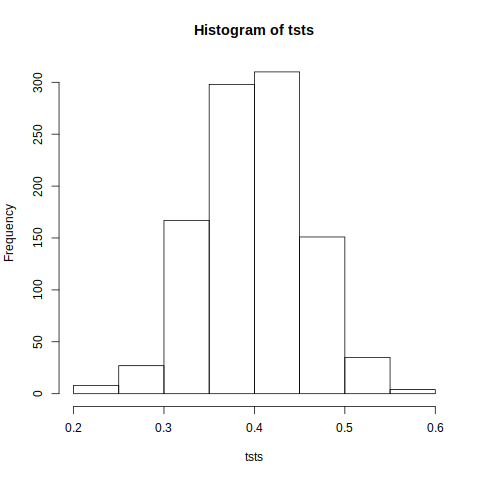
\includegraphics[width=.9\linewidth]{out.png}
\end{center}
\end{document}